\documentclass[11pt]{article}
\usepackage{graphicx,amsmath}
\usepackage{fullpage}
\usepackage[pass]{geometry}
\title{Introduction to topographic surveying and photogrammetry}
\author{Pieter Vermeesch \\Department of Earth Sciences\\ 
        University College London, KLB 116\\
        {\tt p.vermeesch@ucl.ac.uk}}
\date{}
\pagestyle{empty}
\begin{document}
\maketitle
\thispagestyle{empty}

As the name suggests, geomorphology (geo = Earth, morpho = form) is a
field of science concerned with understanding the Earth's
topography. Topographic maps and Digital Elevation Models (DEMs) are
therefore essential tools for geomorphological research. In this
session, we will review the most common techniques to measure
topography, using either land-based observations (Section
\ref{sec:levelling}) or remote sensing (Sections
\ref{sec:photogrammetry}-\ref{sec:SRTM}).

\section{Levelling}
\label{sec:levelling}

The methods introduced in this section can be carried out at low cost
by ground-based individuals.

\subsection{Differential levelling}

This type of survey requires:

\begin{enumerate}
\item A {\it level}, consisting of a telescope and spirit level
  mounted on a tripod.
\item A measuring rod, to be held at a distance of 10-100 metres from
  the level, depending on the steepness of the topography.
\item A point of known elevation, for example an Ordnance Survey Bench
  Mark.
\end{enumerate}

The elevation difference between two points can be mapped by precisely
measuring the vertical distance along a measuring rod held at some
distance from the level (Figure \ref{fig:difflevel}). The survey is
typically done along a closed loop, beginning and ending at the same
bench mark.  To estimate the precision of the resulting elevations, we
simply divide the mismatch between the start and the end of the loop
by the number of measurements in the survey.

\begin{figure}[!ht]
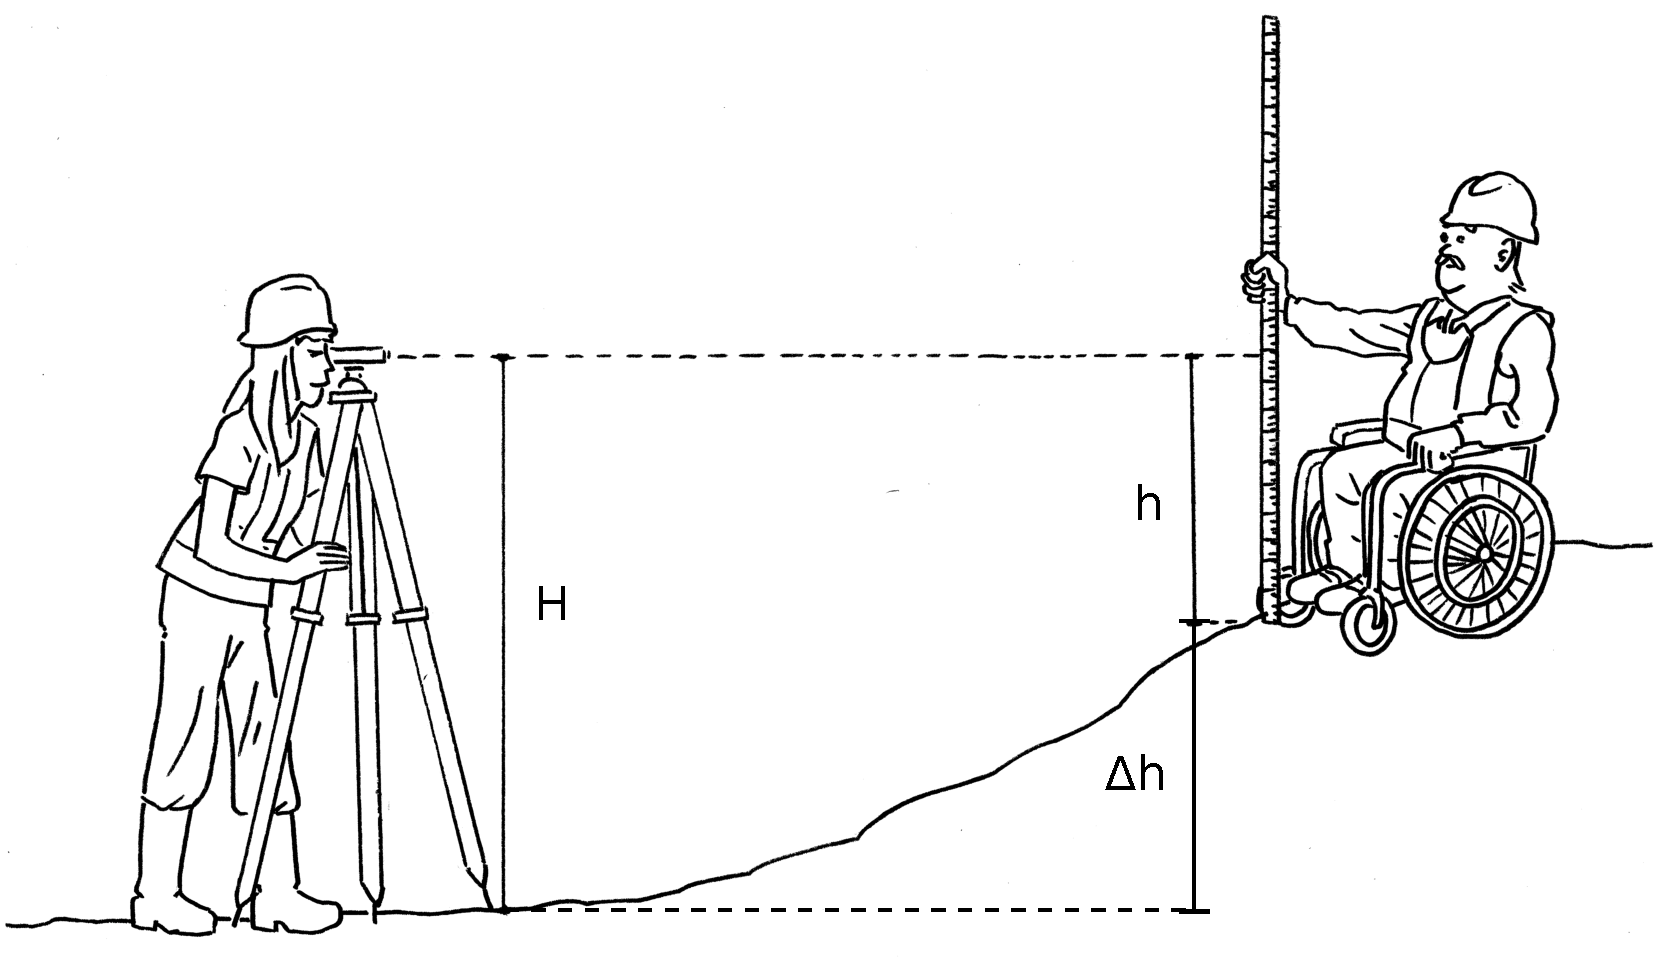
\includegraphics[]{levelling.pdf}
\caption{Differential levelling. The height difference $\Delta h =
  H-h$.}
\label{fig:difflevel}
\end{figure}

\subsection{Trigonometric levelling}
\label{sec:trigonometric}

Differential levelling is very effective in areas of relatively gentle
topography.  However, topographic slopes of greater than 5\% result in
impractically small horizontal steps.  This limitation can be overcome
by using a {\it theodolite} to precisely measure angles to the
horizontal over long distances (Figure \ref{fig:triglevel}). Looking
at the same distant object from two different locations separated by a
known horizontal distance, their viewing angles will differ due to the
parallex effect (see Section \ref{sec:parallax}). Let $\alpha_1$ be
the viewing angle relative to the horizontal plane at location 1 and
$\alpha_2$ the viewing angle at location 2. Let $D$ and $h$ be the
unknown horizontal and vertical distances, respectively, from location
2 to the point of interest, and ($D+d$) the horizontal distance from
location 1.  Then

\begin{align}
& h = D ~\tan(\alpha_2) = (D + d) ~\tan(\alpha_1) \\
& \Rightarrow D ~[\tan(\alpha_2) - \tan(\alpha_1)] = d ~\tan(\alpha_1) \\
& \Rightarrow D = d ~\tan(\alpha_1)~/~[\tan(\alpha_2) - \tan(\alpha_1)] \\
& \Rightarrow h = d ~\tan(\alpha_1) ~ \tan(\alpha_2)~/~[\tan(\alpha_2) - \tan(\alpha_1)]
\end{align}

\begin{figure}[!ht]
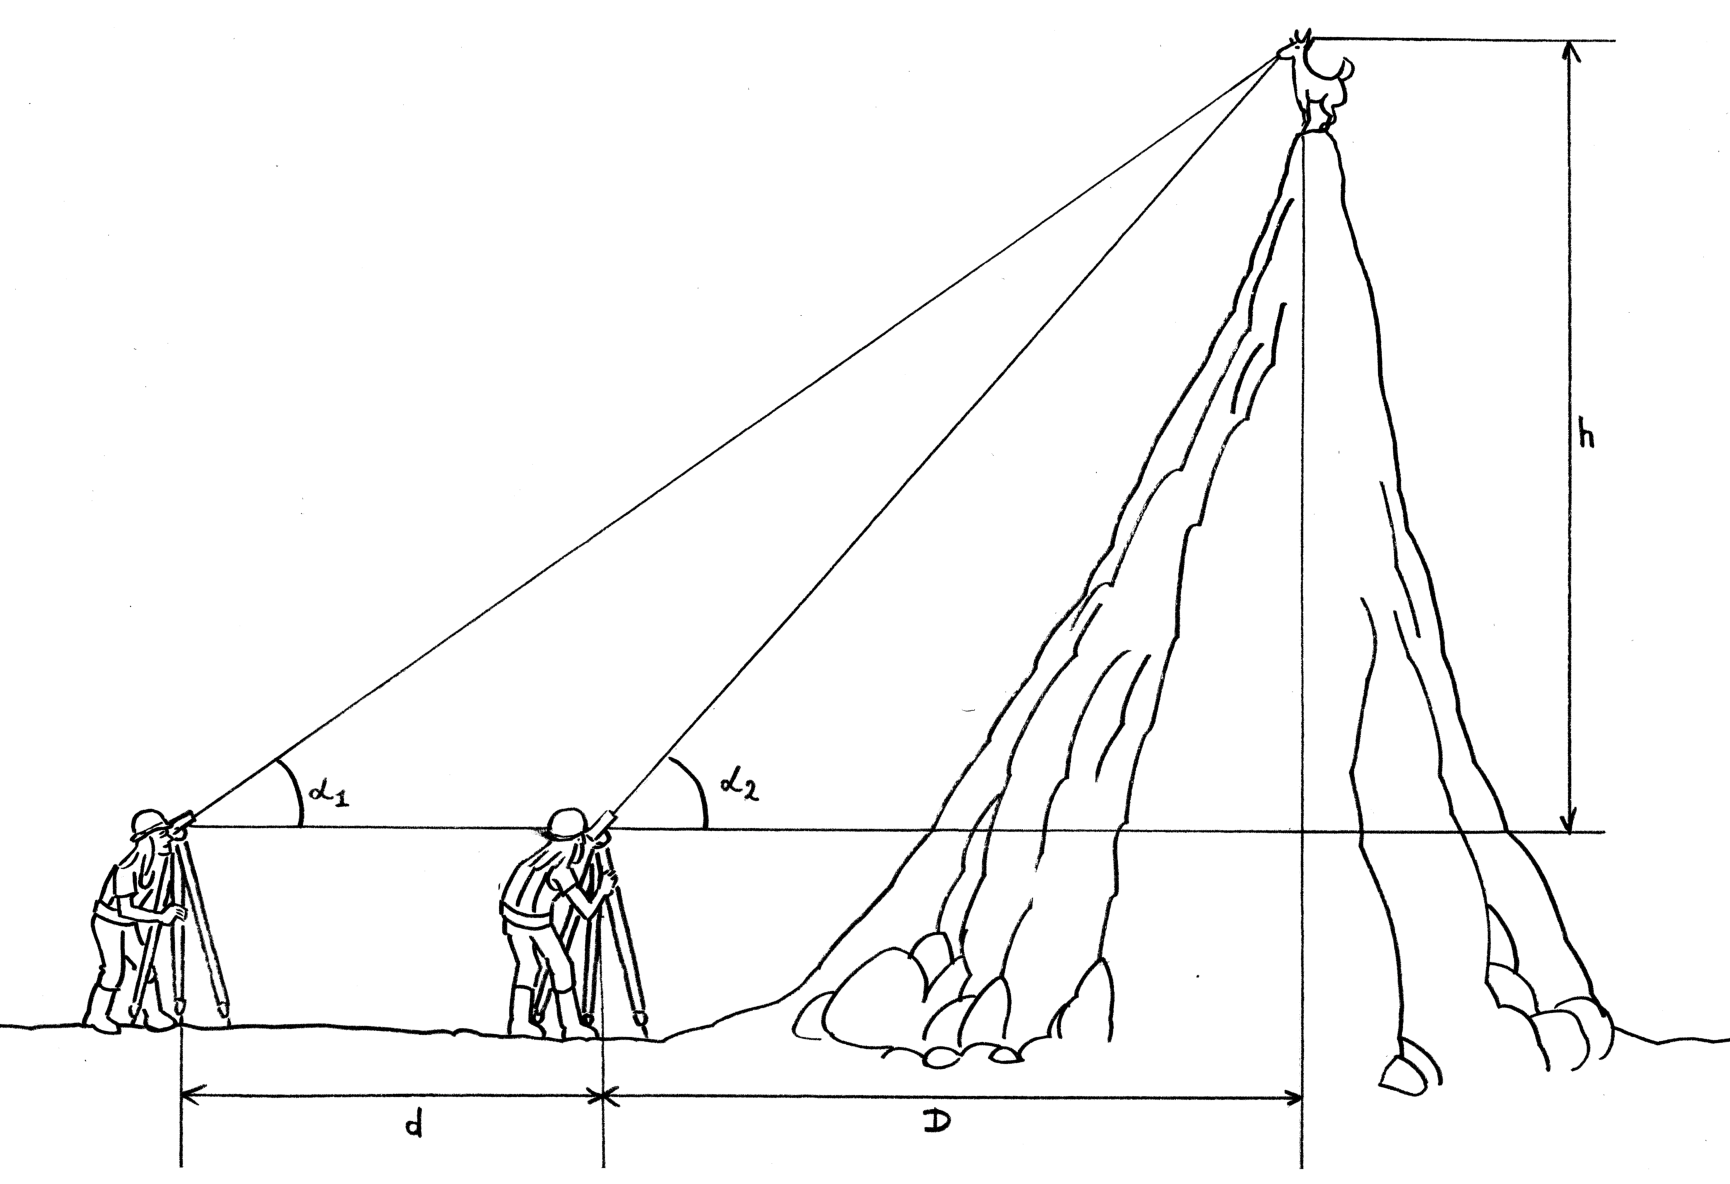
\includegraphics[]{difflevelling.pdf}
\caption{Trigonometric levelling}
\label{fig:triglevel}
\end{figure}

\noindent\emph{exercise:}

\noindent You stand on a level beach and look up to the edge of
a cliff above. The viewing angle is 60\textsuperscript{$\circ$}.
Stepping back 10 m, the viewing angle reduces to
50\textsuperscript{$\circ$}.  How high is the cliff?

\subsection{Barometric levelling}

Water is an {\it incompressible} fluid, and so its pressure ($P$)
increases linearly with depth ($z$):

\begin{equation}
P = \rho ~ g ~ z
\label{eq:water}
\end{equation}

where $\rho$ is the density of water ($\sim$ 1 kg/l) and $g$ is the
gravitational constant ($\sim$9.81 m/s$^2$). Scuba-divers use Equation
\ref{eq:water} to determine the depth of their dives. Likewise,
mountaineers can use air pressure to determine elevation
($h$). However, because air is a {\it compressible} fluid, they cannot
use Equation \ref{eq:water}, but must employ a different formula:

\begin{equation}
P = P_\circ e^{-h/8435}
\label{eq:air}
\end{equation}

where $P_\circ$ is the pressure at sea level ($\sim$ 1013.25 mbar) and
8435 is the {\it e-folding length} of the exponential function, in
metres.  Using Equation \ref{eq:air}, we can calculate that the air
pressure on the summit of Mount Makalu (close to 8435m high) is
approximately 2.71 ($= e$) times lower than at sea level. One problem with
barometric elevation surveys is the variability of $P_\circ$, which
can range from 980 mbar (low pressure, bad weather) to 1050 mbar (high
pressure, good weather), potentially resulting in up to

\begin{equation}
\Delta h = 8435 ~ \ln(1050/980) = 582
\end{equation}

metres of variability in `apparent elevation'. It is therefore
important to calibrate the barometer to the elevation of a bench mark
before (and after) a barometric survey.

\subsection{(differential) GPS}

The Global Positioning System (GPS) measures the horizontal and
vertical location of GPS receivers relative to a constellation of
satellites.  The positional accuracy is greatly improved by monitoring
the relative distances (both horizontally and vertically) relative to
a fixed GPS receiver, located at a known location (e.g. a bench
mark). This is called {\it differential} GPS and has allowed
geodesists to monitor plate tectonic movements with millimetre
accuracy and precision.

\section{Photogrammetry}
\label{sec:photogrammetry}

Levelling surveys are restricted to individual point measurements or
profiles. The following methods overcome this limitation and cover
large continuous areas using photographs, taken from above.

\subsection{Single image}

It is possible to obtain the height of vertical objects such as trees,
buildings or cliff faces from a single aerial photograph (Figure
\ref{fig:singleimage}).  Define the {\it principal point} of an aerial
photograph as the point located directly below the airplane.  Let $D$
be the measured horizontal distance on the photograph from the
principal point to the top of the object of interest, and let $d$ be
the measured distance on the photograph between its base and its
top. Finally, let $H$ be the height of the airplane above the
ground. Then the height of the object can be calculated as

\begin{equation}
h = H ~ d ~ / D
\end{equation}

\begin{figure}[!ht]
  \centering
  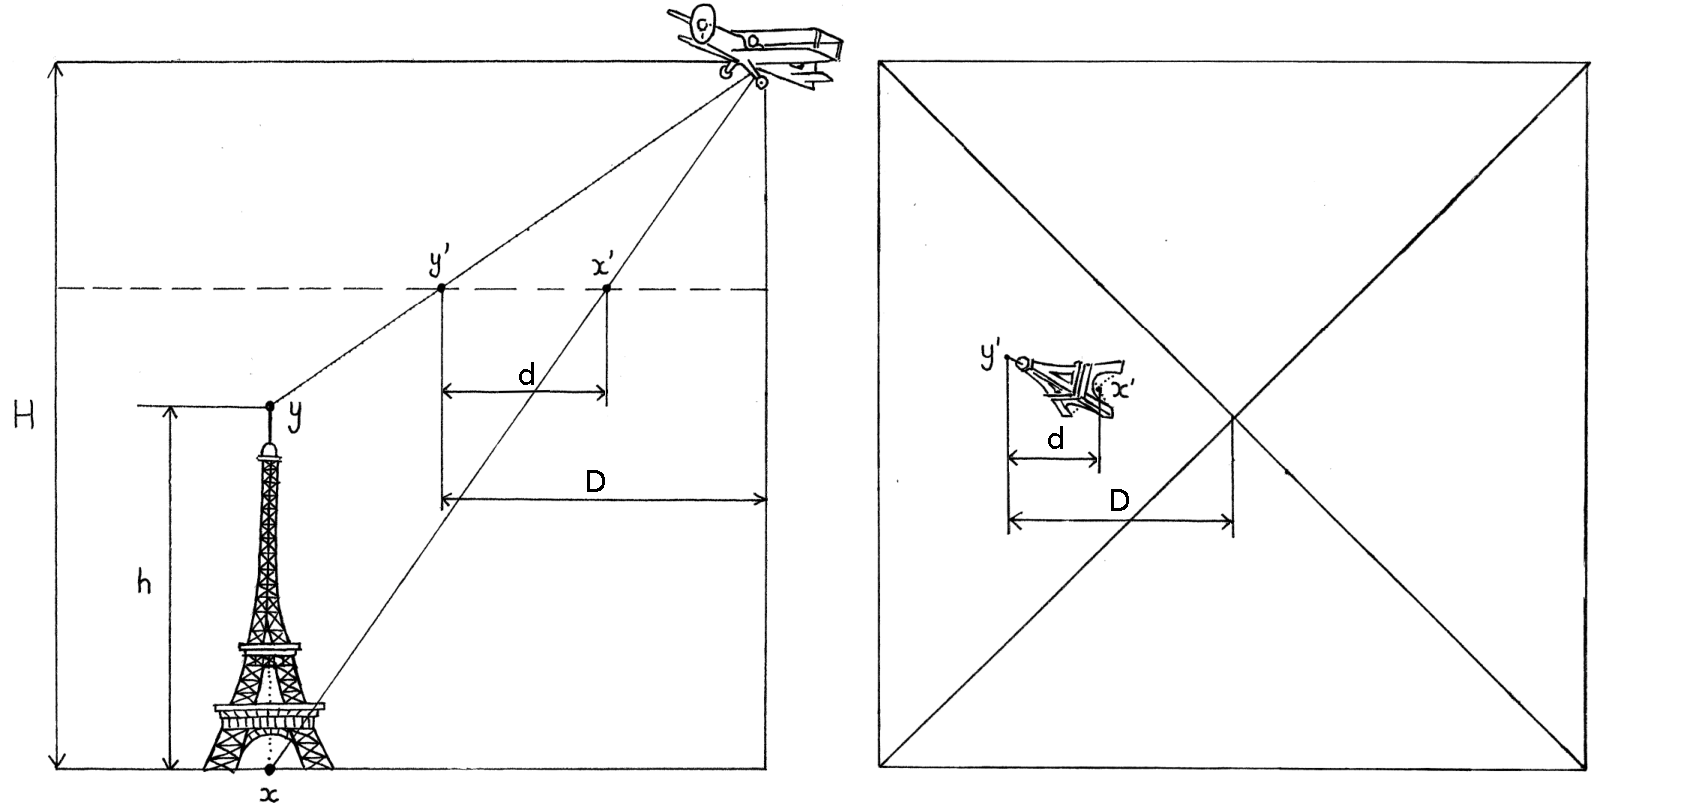
\includegraphics[]{single-image.pdf}
  \caption{Photogrammetry from a single image.}
  \label{fig:singleimage}
\end{figure}

\noindent\emph{exercise:}

\noindent Estimate the height of the cooling towers shown in aerial
photograph B at the end of these notes, which was taken at an altitude
of 1000m.

\subsection{Stereo-imagery}
\label{sec:parallax}

\begin{figure}[!ht]
  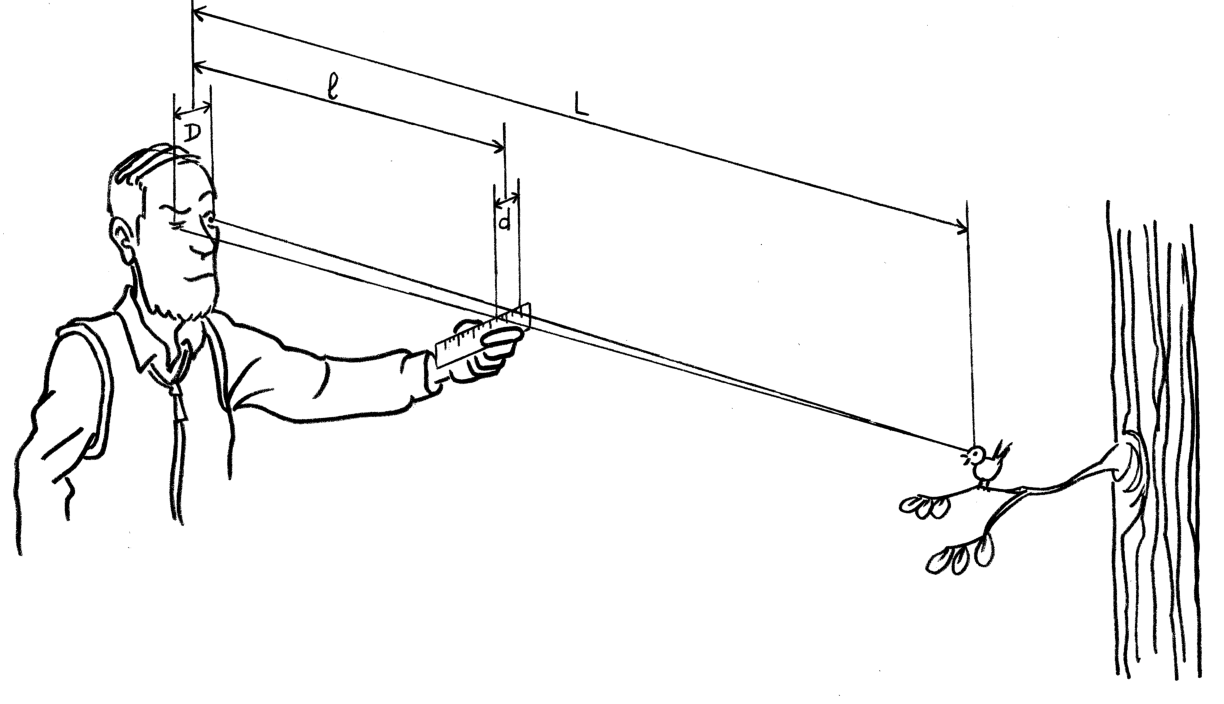
\includegraphics[]{parallax.pdf}
  \caption{The parallax effect is used by the human brain to perceive
    depth.}
  \label{fig:parallax}
\end{figure}

Single images can only be used to measure vertical objects. This
limitation can be overcome by using two images taken at different
locations, and utilising the parallax effect (see Section
\ref{sec:trigonometric}). To illustrate this effect, carry out the
following experiment (Figure \ref{fig:parallax}):

\begin{enumerate}
\item Choose any small object located 2-5 metres away from you, and
  close your right eye.
\item Stretch out your arm, holding a ruler, and align the `zero'
  marker with the object.
\item Open your right eye, close the left one, and note the apparent
  shift in location of your chosen object along the ruler, in
  millimetres ($d$).
\item Measure the length of your arm ($l$) and the distance between
  your eyes ($D$).
\end{enumerate}

Then we can calculate the distance from your eyes to the chosen object as

\begin{equation}
  d / D = (L - l) / L \Rightarrow L = l D / (D - d)
\end{equation}

The same principle is used by astronometers to measure the distance
($L$) from the Earth to other planets and nearby stars (Figure
\ref{fig:astronomy}), using the diameter of Earth's orbit around the
Sun as a baseline ($l$) and the apparent angle from the baseline to
the object of interest as a parallax angle ($\alpha$):

\begin{equation}
  L = l / \tan(\alpha)
  \label{eq:astronomy}
\end{equation}

\begin{figure}[!ht]
  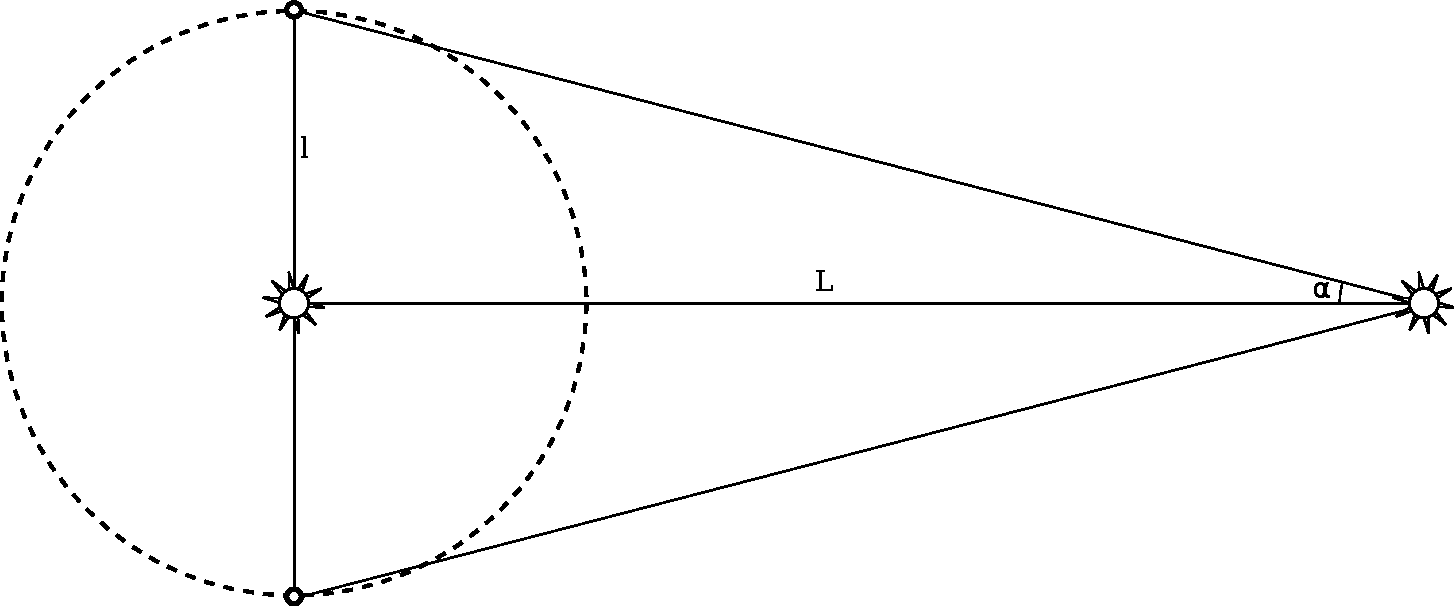
\includegraphics[]{astronomy2.pdf}
  \caption{The orbit of the Earth around the Sun provides a
    sufficiently long baseline from which to observe a measurable
    parallax effect to nearby stars.}
  \label{fig:astronomy}
\end{figure}

\noindent\emph{exercise:}

\noindent A \emph{parsec} is the physical distance to a celestial
object for which $\alpha$ = 1 arc second in Equation
\ref{eq:astronomy}. Given that light travels from the Sun to Earth in
8 minutes and 20 seconds, how many light years does one parsec equal
to?\\

Given a {\it stereo-set} of two aerial photographs (or satellite
images), we can determine the elevation distance between any two
points x and y (not just those located immediately above or below each
other) as follows:

\begin{enumerate}
\item Determine the horizontal distances from the principal point of
  image A to points x and y ($p_x(A)$ and $p_y(A)$, respectively).  Do
  the same for image B ($p_x(B)$ and $p_y(B)$).
\item Calculate the {\it parallax} of points $x$ and $y$ as

\begin{align}
& p_x = p_x(A) - p_x(B)\\
& p_y = p_y(A) - p_y(B)
\end{align}

\item If the images were taken at an altitude $H$, then the
elevation difference between points $x$ and $y$ is given by

\begin{equation}
h = H ~ (p_y - p_x) ~/~ p_y
\end{equation}
\end{enumerate}

\begin{figure}[!ht]
  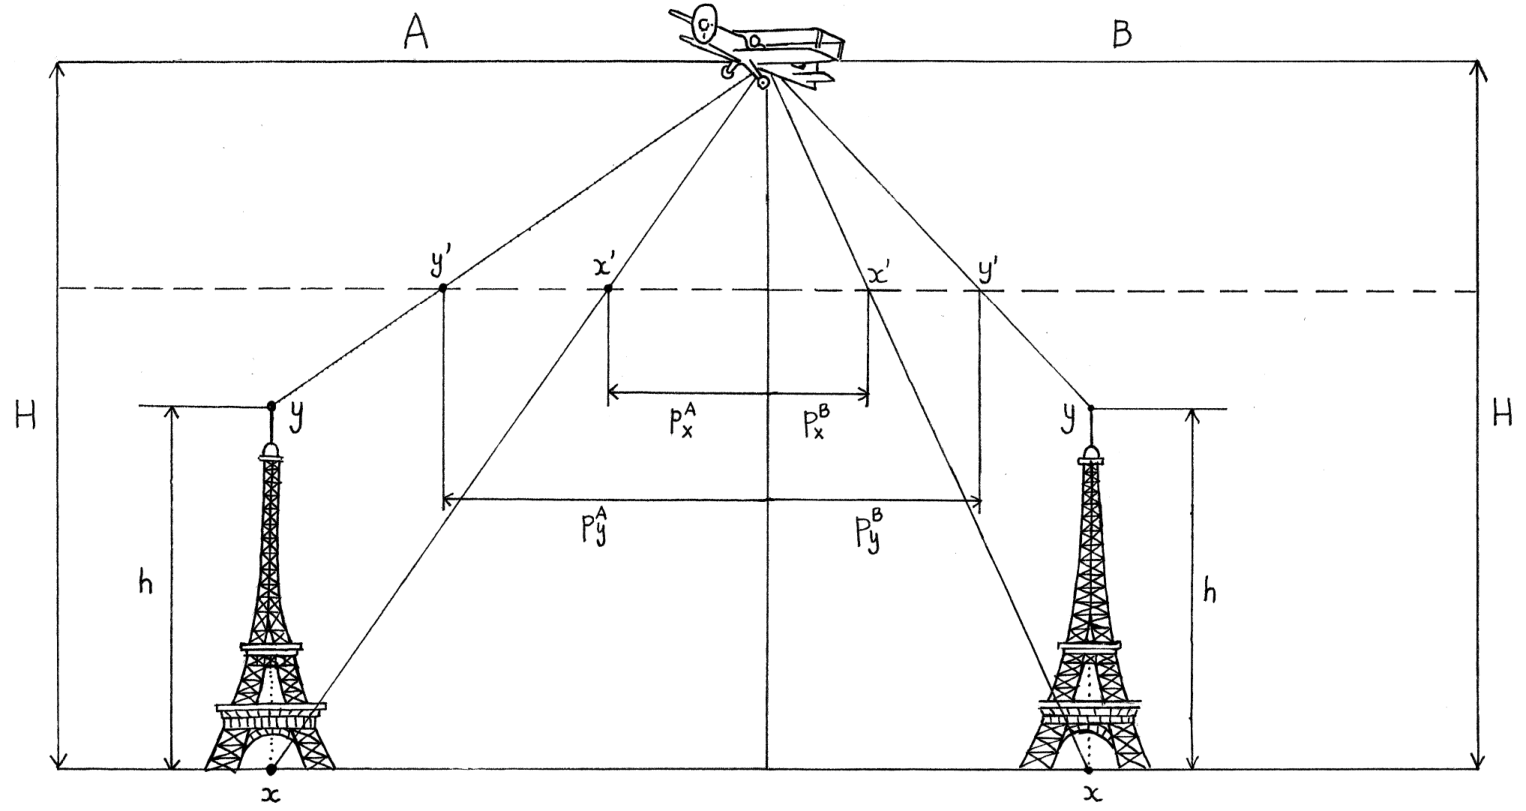
\includegraphics[]{stereo1.pdf}\\
  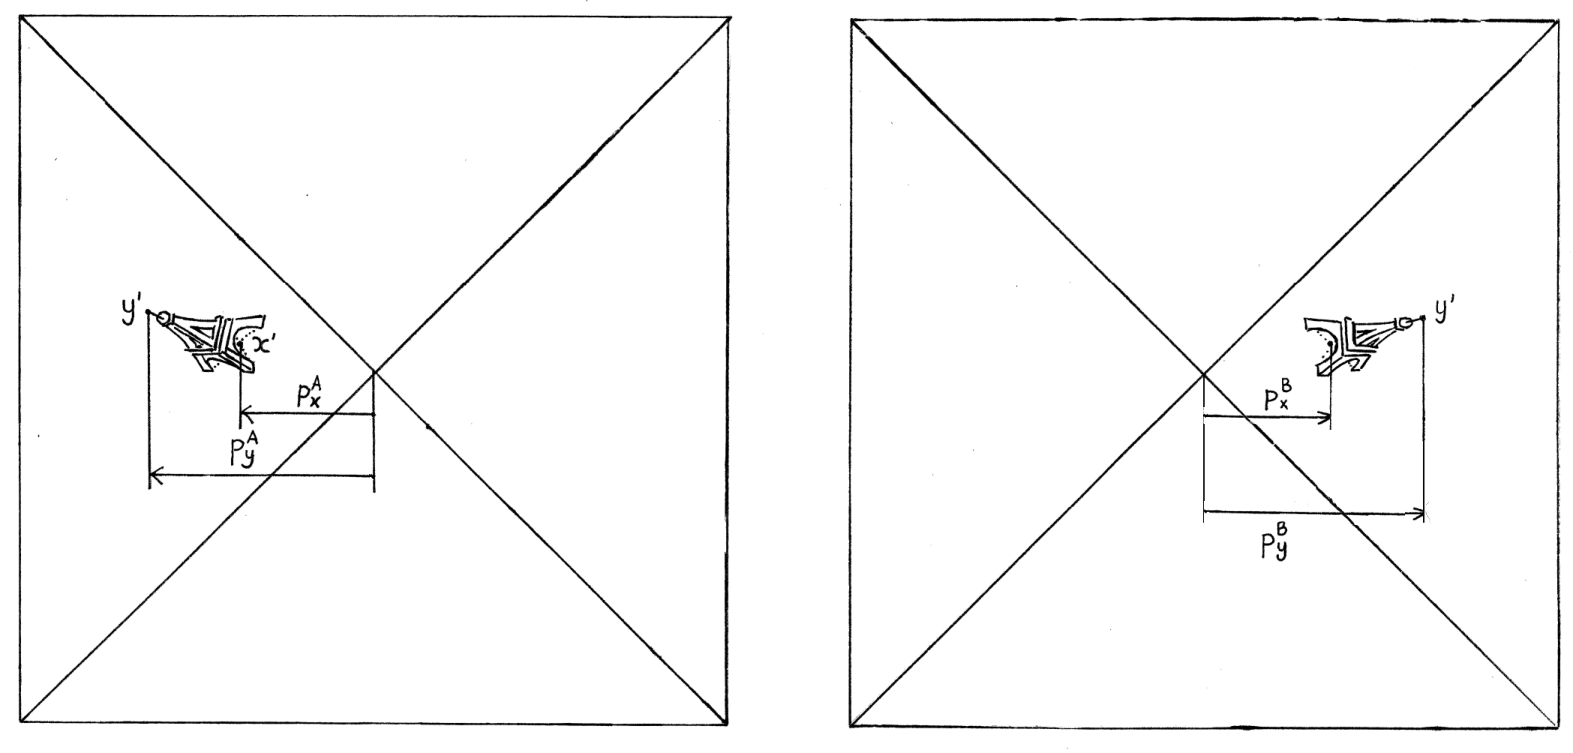
\includegraphics[]{stereo2.pdf}
  \caption{Photogrammetry with stereo-images. Note that $p_x^A$,
    $p_x^B$, $p_y^A$ and $p_y^B$ can be either positive or negative.}
  \label{fig:stereo}
\end{figure}

Topographic contour maps are created by connecting points of equal
parallax on a stereo-image, using a {\it parallax bar}.\\

\noindent\emph{exercise:}

\noindent Calculate the height of the cooling towers (last page of
these notes) using the principles of stereo-photogrammetry, again
assuming that the photographs were taken at an altitude of 1000m.

\section{Lidar}

Lidar stands for `LIght Detection And Ranging' and is based on similar
principles to sonar (`SOund Navigation And Ranging') and radar (`RAdio
Detection And Ranging'). It determines elevation ($h$) by measuring
the two-way travel time ($\Delta t$) of short light pulses between an
airborne light source and the ground (Figure \ref{fig:lidar}):

\begin{equation}
h = v ~ \Delta t ~ / ~ 2
\end{equation}

where $v$ is the speed of light ($\sim$ 3 $\times$10$^8$m/s). Two-way
travel times can be measured with a precision of $\sim$ 1 ns. Can you
work out the vertical resolution of Lidar?

\begin{figure}[!ht]
  \centering
  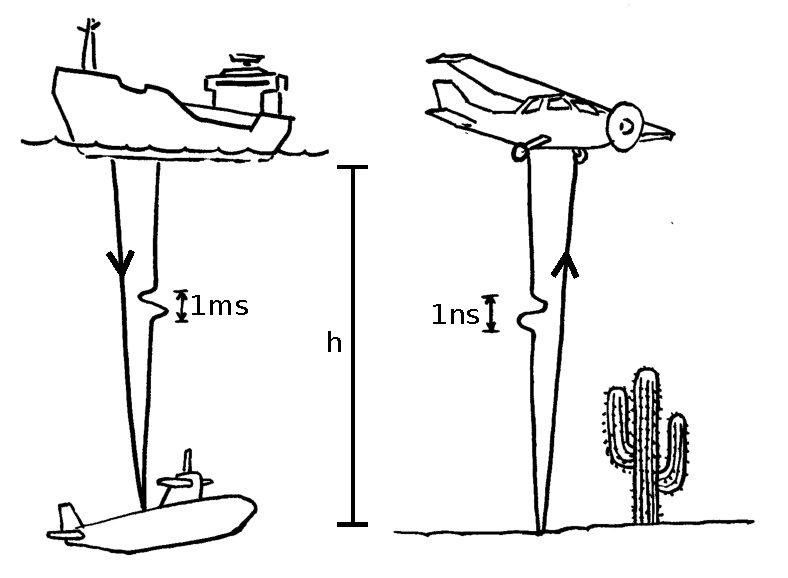
\includegraphics[width=.5\textwidth]{lidar.pdf}
  \caption{Sonar, lidar (and radar) are all based on the same principles.}
  \label{fig:lidar}
\end{figure}

\section{SRTM}
\label{sec:SRTM}

During 11 days in February 2000, space shuttle Endeavor carried out
the Shuttle Radar Topography Mission (SRTM). Using a radar (microwave)
source and two detectors separated by a distance of 60 m, it circled
the Earth, recording the interference patterns of the reflected light
(Figure \ref{fig:SRTM}).  The resulting data went through several
stages of post-processing, ultimately resulting in a Digital Elevation
Model (DEM) with near-global coverage and a horizontal resolution of
30m. The data are available free of charge at {\tt
  http://srtm.csi.cgiar.org/}

\begin{figure}[!ht]
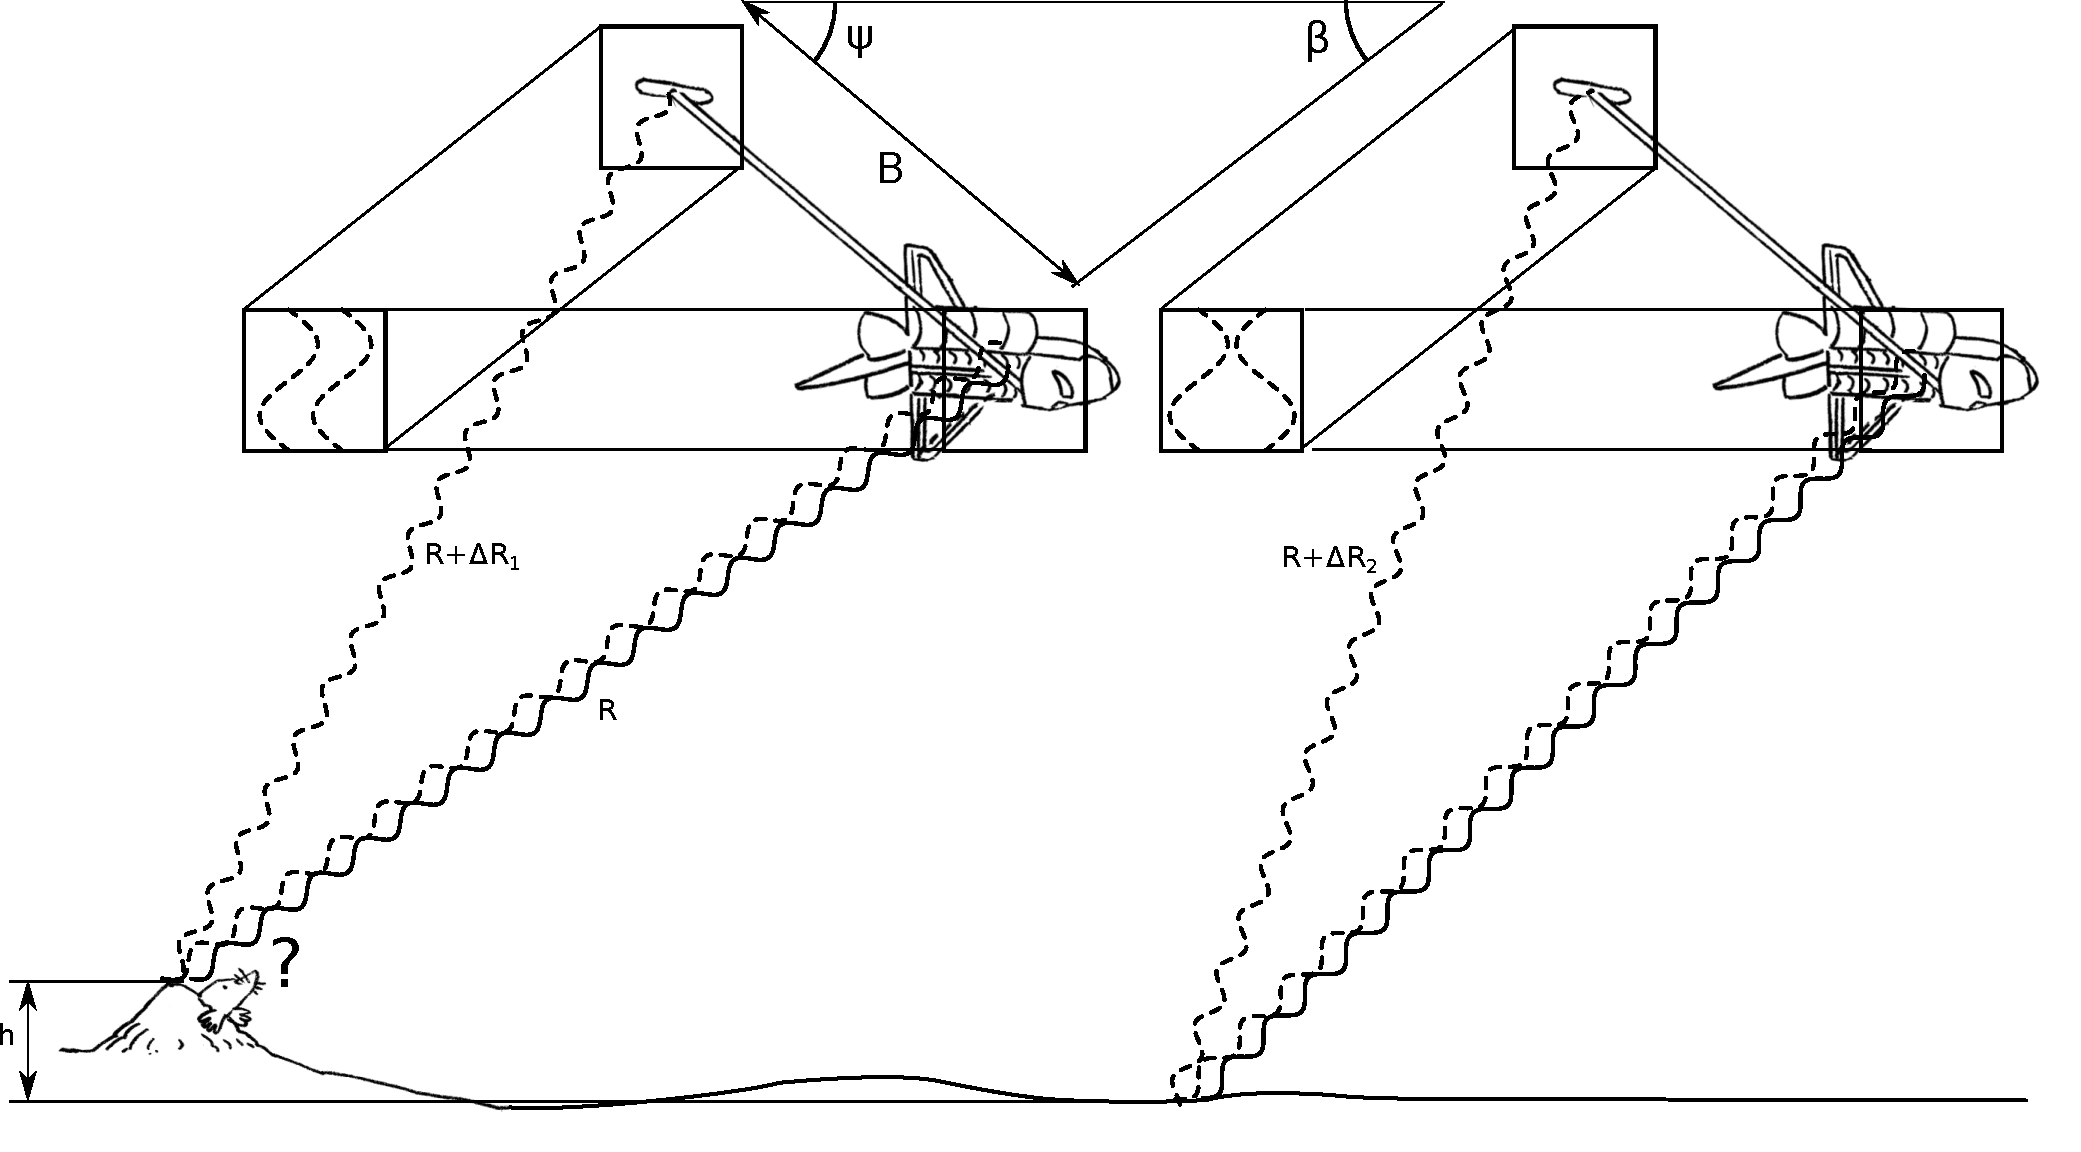
\includegraphics[]{SRTM.pdf}
\caption{SRTM uses the principles of interferometry, in which a radar
  source (solid lines) emits electromagnetic radiation to the surface,
  which is reflected (dashed lines) by the Earth and received by two
  receivers, offset by a baseline distance B (= 60m). Changes in range
  ($\Delta R$) are determined by monitoring the phase of the incoming
  radar waves. Thus, the left and right images exhibit destructive and
  constructive interference, respectively. Differences in height ($h$)
  can be obtained using the following formula: $ h \approx ( R / B )
  (\Delta R_2 - \Delta R_1) \cos(\psi) / \sin(\psi+\beta) $ }
\label{fig:SRTM}
\end{figure}

\clearpage

\begin{figure}[!ht]
  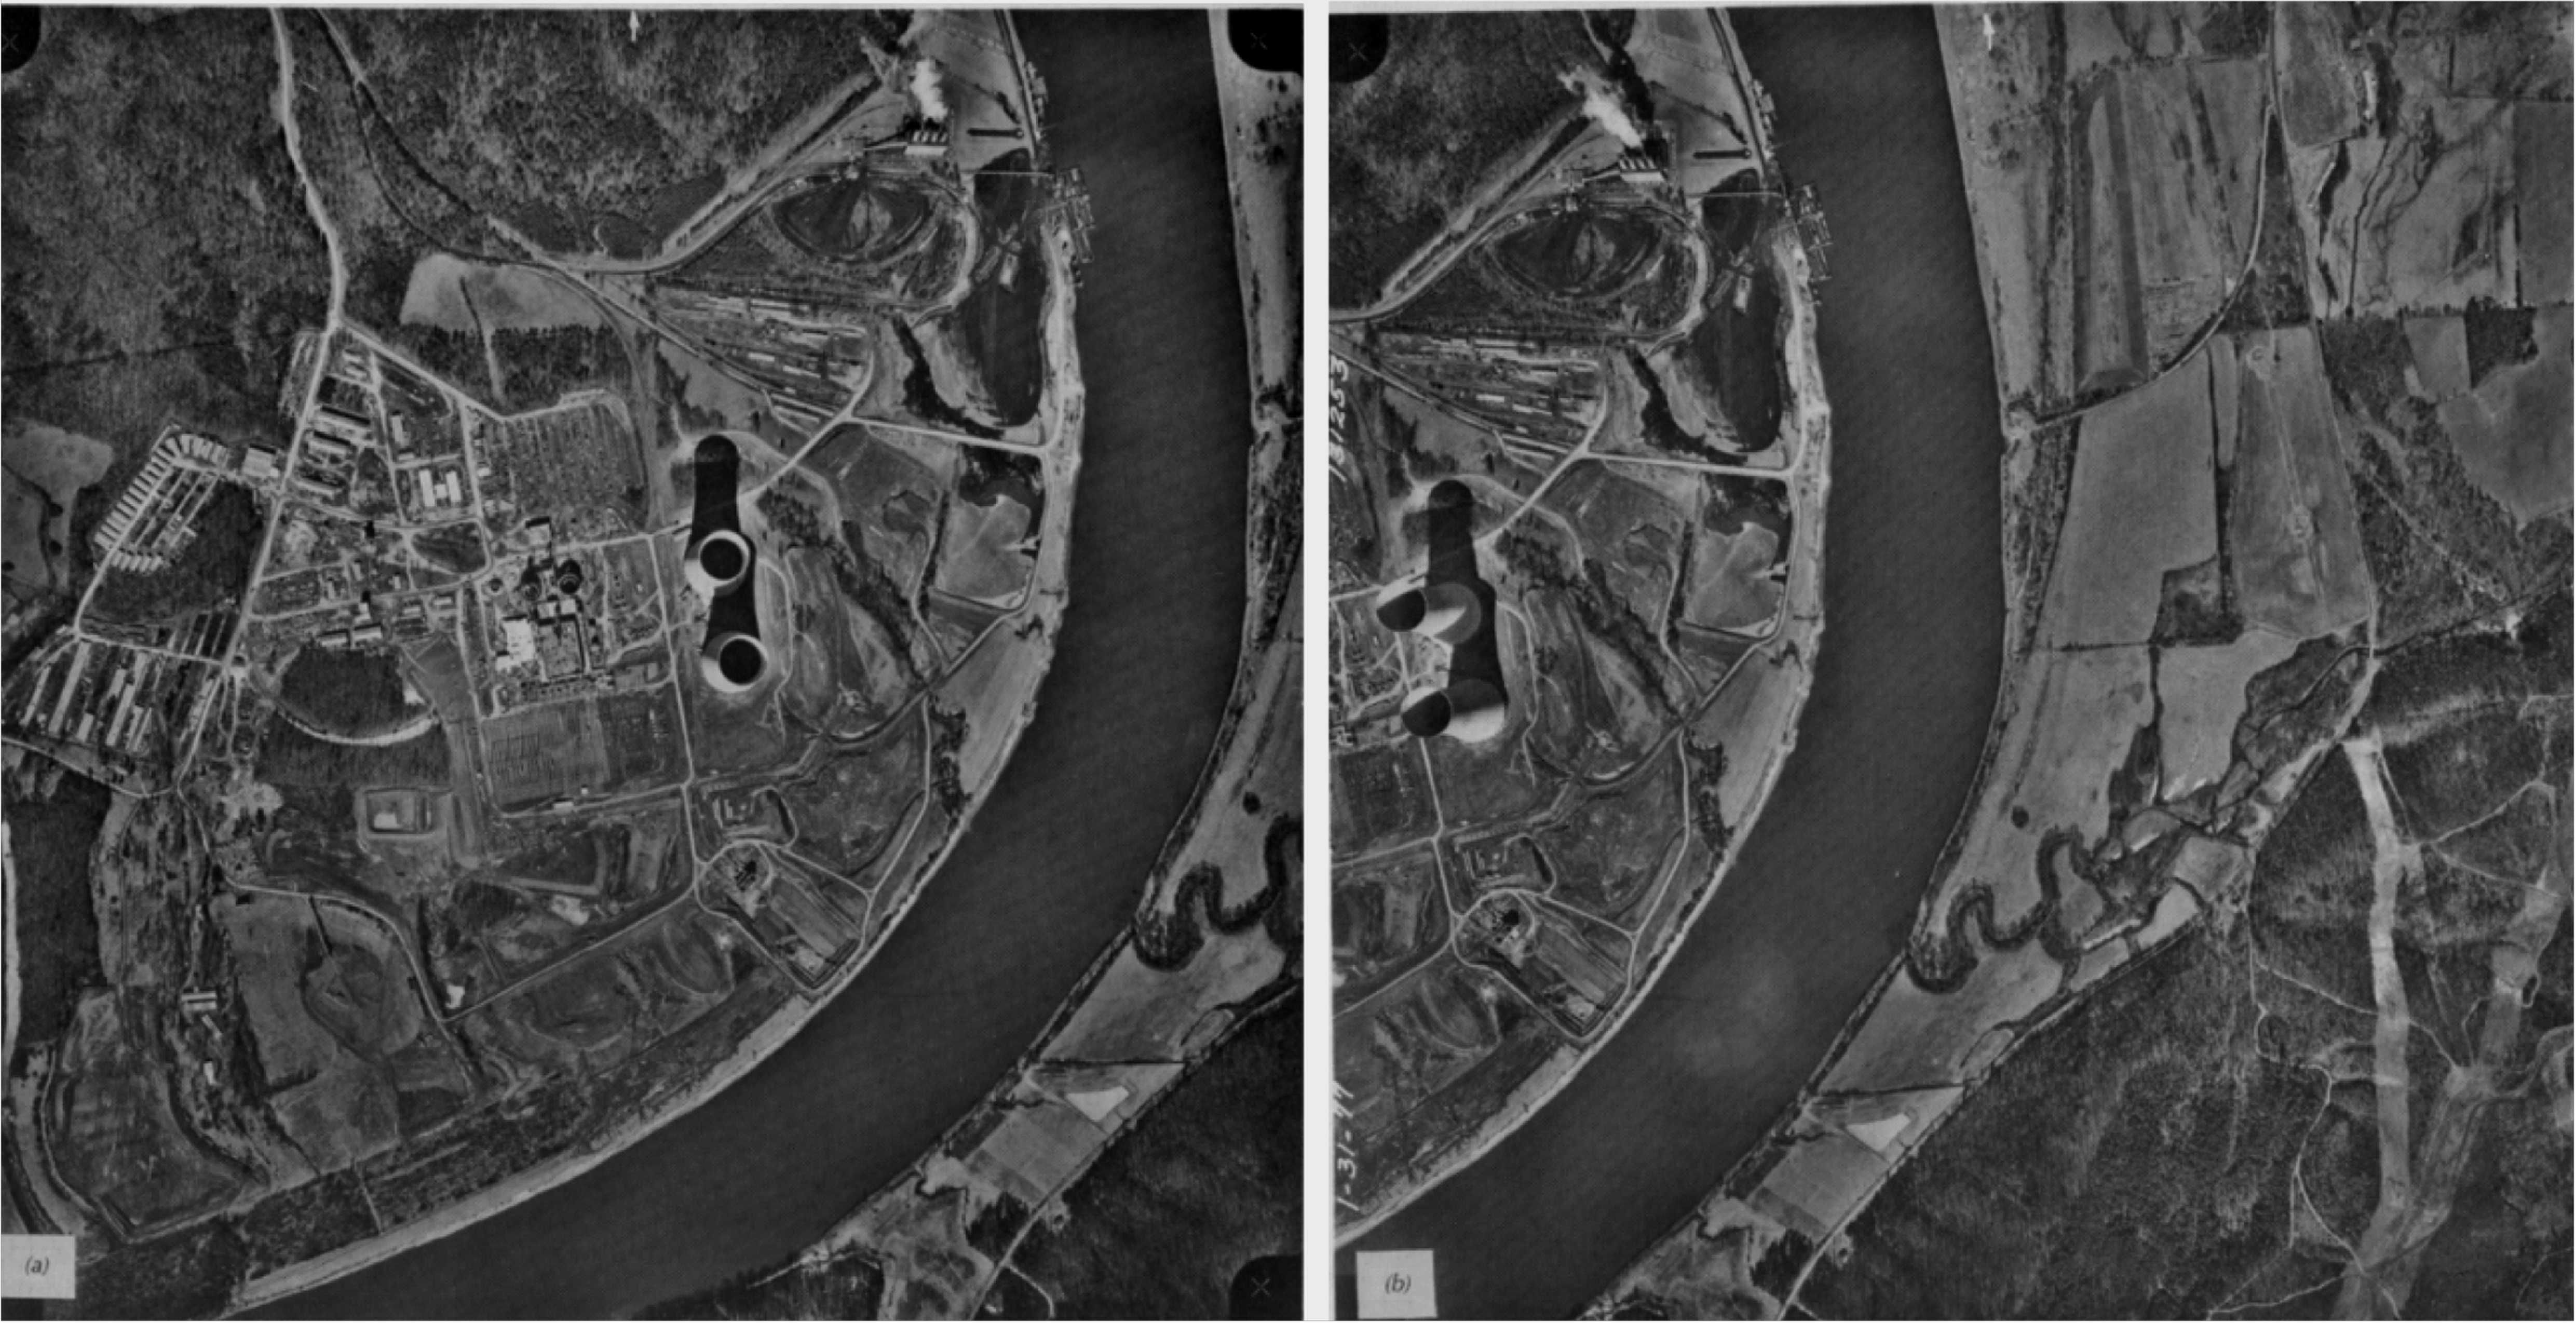
\includegraphics[]{cooling-towers.pdf}
  \label{fig:cooling}
\end{figure}

\end{document}
